\chapter{Function GumbelUnc.mat}


\begin{figure}[H]
\center
\fbox{
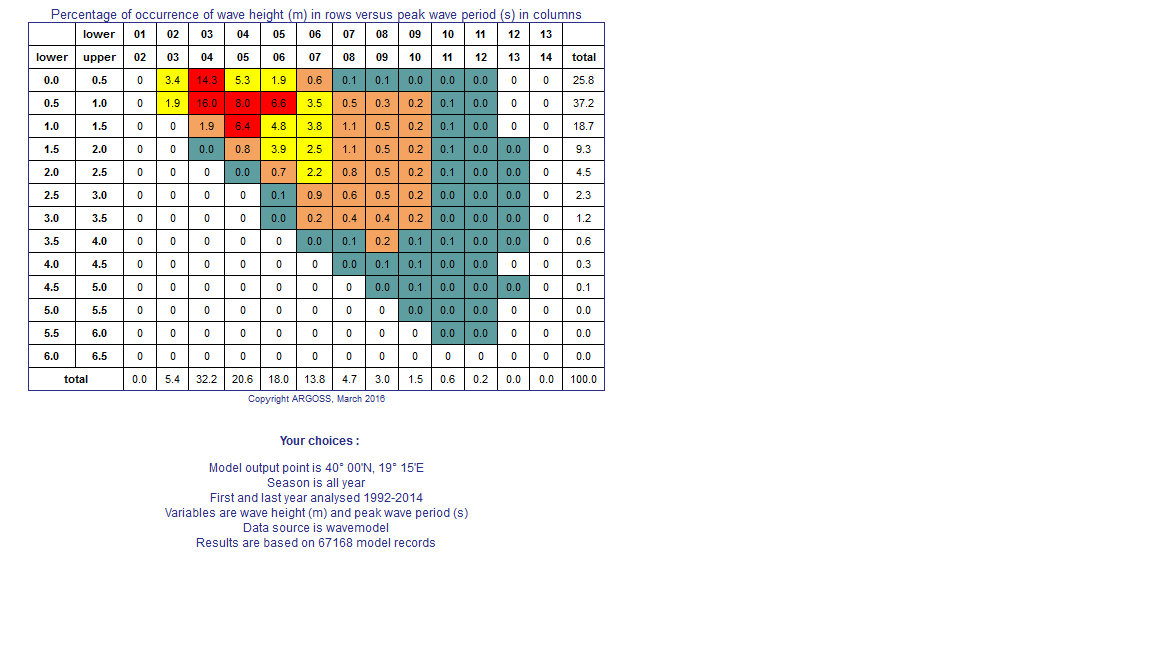
\includegraphics[width=\textwidth]{images/wave_pperiod_allyear.png} 
}
\caption[Distribution of peak-period over wave hight]{Distribution of peak-period over wave hight}
%\label{Distribution_pperiod}
\end{figure}


\begin{figure}[H]
\center
\fbox{
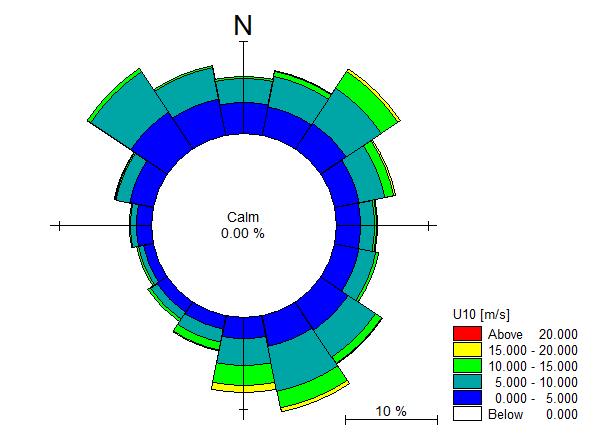
\includegraphics[width=\textwidth]{images/Rose_plot_u10.png} 
}
\caption[Rose-diagram with the distribution of the wind}
%\label{Windrose}
\end{figure}


\begin{figure}[H]
\center
\fbox{
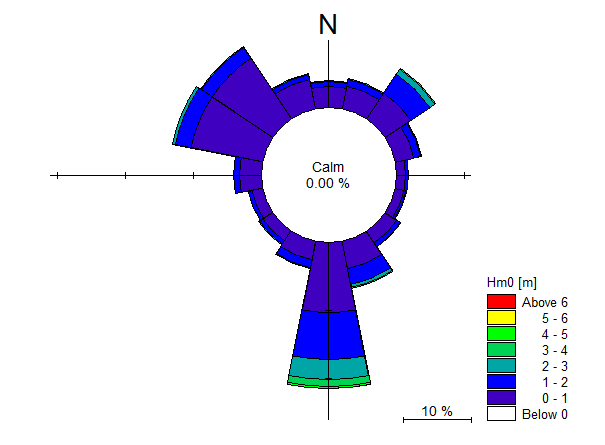
\includegraphics[width=\textwidth]{images/Rose_plot_Hoverall.png} 
}
\caption[Rose-diagram with the distribution of the waves}
%\label{wavedata_angle}
\end{figure}
Whatever XX
